\pdfbookmark{Общая характеристика работы}{characteristic}             % Закладка pdf
\section*{Общая характеристика работы}

\newcommand{\actuality}{\pdfbookmark[1]{Актуальность}{actuality}\underline{\textbf{\actualityTXT}}}
\newcommand{\progress}{\pdfbookmark[1]{Разработанность темы}{progress}\underline{\textbf{\progressTXT}}}
\newcommand{\aim}{\pdfbookmark[1]{Цели}{aim}\underline{{\textbf\aimTXT}}}
\newcommand{\tasks}{\pdfbookmark[1]{Задачи}{tasks}\underline{\textbf{\tasksTXT}}}
\newcommand{\aimtasks}{\pdfbookmark[1]{Цели и задачи}{aimtasks}\aimtasksTXT}
\newcommand{\novelty}{\pdfbookmark[1]{Научная новизна}{novelty}\underline{\textbf{\noveltyTXT}}}
\newcommand{\influence}{\pdfbookmark[1]{Практическая значимость}{influence}\underline{\textbf{\influenceTXT}}}
\newcommand{\methods}{\pdfbookmark[1]{Методология и методы исследования}{methods}\underline{\textbf{\methodsTXT}}}
\newcommand{\defpositions}{\pdfbookmark[1]{Положения, выносимые на защиту}{defpositions}\underline{\textbf{\defpositionsTXT}}}
\newcommand{\reliability}{\pdfbookmark[1]{Достоверность}{reliability}\underline{\textbf{\reliabilityTXT}}}
\newcommand{\probation}{\pdfbookmark[1]{Апробация}{probation}\underline{\textbf{\probationTXT}}}
\newcommand{\contribution}{\pdfbookmark[1]{Личный вклад}{contribution}\underline{\textbf{\contributionTXT}}}
\newcommand{\publications}{\pdfbookmark[1]{Публикации}{publications}\underline{\textbf{\publicationsTXT}}}


{\actuality} 
В настоящее время диссипативные квантовые системы являются неотъемлемой частью экспериментальной и технологической реальности.
Практические реализации нано- \autocite{Poot2012} и опто-механических систем \autocite{Aspelmeyer2014}, сверхпроводящих элементов \autocite{Clarke2008} не осуществимы в полной изоляции от окружающей среды.
Эволюция идеальных когерентных квантовых систем является простым приближением реальных физических процессов. 
Все эти системы являются открытыми и их динамика существенно диссипативна.
Диссипация в данных системах является полноправным генератором эволюции, которая не менее сложна и разнообразна, чем унитарная, генерируемая гамильтонианами.
Асимптотические состояния открытых квантовых систем определится не только гамильтоновой динамикой, но взаимодействием с окружающей средой.
Данное взаимодействие не является достаточно сильным, чтобы полностью свести динамику системы к классическому случаю \autocite{Breuer2007}.
Особенностью диссипации является то, что она способна привести систему в состояния, которые недостижимы в классическом пределе.
Например, новые топологические состояния, получаемые за счёт управляемой синтетической диссипации \autocite{Diehl2011} или «чистые» сильно запутанные состояния в многочастичных квантовых системах \autocite{Kraus2008}.

На сегодняшний день теория открытых квантовых систем является хорошо развитой областью теоретической физики с широким спектром разноплановых фундаментальных результатов и методов \autocite{Breuer2007}.
Одним из самых распространённых подходов к описанию динамики открытых квантовых систем является формализм Линдблада \autocite{Lindblad1976, Gorini1976}

Наиболее мощным и исследованным подходом является
формализм Линдблада, который основан на идеях квантовых динамических полугрупп [7]
и идеологии квантовых скачков, особенно популярной в квантовой оптике [8,9,10]. Этот
подход также широко используется в контексте оптомеханики и квантовых
электродинамических систем (КЭД); отметим также приложения в физике холодных
атомов [5,11,12].




 
Обзор, введение в тему, обозначение места данной работы в
мировых исследованиях и~т.\:п., можно использовать ссылки на~другие
работы~\autocite{Gosele1999161,Lermontov}
(если их~нет, то~в~автореферате
автоматически пропадёт раздел <<Список литературы>>). Внимание! Ссылки
на~другие работы в~разделе общей характеристики работы можно
использовать только при использовании \verb!biblatex! (из-за технических
ограничений \verb!bibtex8!. Это связано с тем, что одна
и~та~же~характеристика используются и~в~тексте диссертации, и в
автореферате. В~последнем, согласно ГОСТ, должен присутствовать список
работ автора по~теме диссертации, а~\verb!bibtex8! не~умеет выводить в~одном
файле два списка литературы).
При использовании \verb!biblatex! возможно использование исключительно
в~автореферате подстрочных ссылок
для других работ командой \verb!\autocite!, а~также цитирование
собственных работ командой \verb!\cite!. Для этого в~файле
\verb!common/setup.tex! необходимо присвоить положительное значение
счётчику \verb!\setcounter{usefootcite}{1}!.

Для генерации содержимого титульного листа автореферата, диссертации
и~презентации используются данные из файла \verb!common/data.tex!. Если,
например, вы меняете название диссертации, то оно автоматически
появится в~итоговых файлах после очередного запуска \LaTeX. Согласно
ГОСТ 7.0.11-2011 <<5.1.1 Титульный лист является первой страницей
диссертации, служит источником информации, необходимой для обработки и
поиска документа>>. Наличие логотипа организации на~титульном листе
упрощает обработку и~поиск, для этого разметите логотип вашей
организации в папке images в~формате PDF (лучше найти его в векторном
варианте, чтобы он хорошо смотрелся при печати) под именем
\verb!logo.pdf!. Настроить размер изображения с логотипом можно
в~соответствующих местах файлов \verb!title.tex!  отдельно для
диссертации и автореферата. Если вам логотип не~нужен, то просто
удалите файл с~логотипом.

\ifsynopsis
Этот абзац появляется только в~автореферате.
Для формирования блоков, которые будут обрабатываться только в~автореферате,
заведена проверка условия \verb!\!\verb!ifsynopsis!.
Значение условия задаётся в~основном файле документа (\verb!synopsis.tex! для
автореферата).
\else
Этот абзац появляется только в~диссертации.
Через проверку условия \verb!\!\verb!ifsynopsis!, задаваемого в~основном файле
документа (\verb!dissertation.tex! для диссертации), можно сделать новую
команду, обеспечивающую появление цитаты в~диссертации, но~не~в~автореферате.
\fi

% {\progress}
% Этот раздел должен быть отдельным структурным элементом по
% ГОСТ, но он, как правило, включается в описание актуальности
% темы. Нужен он отдельным структурынм элемементом или нет ---
% смотрите другие диссертации вашего совета, скорее всего не нужен.

{\aim} данной работы является \ldots

Для~достижения поставленной цели необходимо было решить следующие {\tasks}:
\begin{enumerate}[beginpenalty=10000] % https://tex.stackexchange.com/a/476052/104425
  \item Исследовать, разработать, вычислить и~т.\:д. и~т.\:п.
  \item Исследовать, разработать, вычислить и~т.\:д. и~т.\:п.
  \item Исследовать, разработать, вычислить и~т.\:д. и~т.\:п.
  \item Исследовать, разработать, вычислить и~т.\:д. и~т.\:п.
\end{enumerate}


{\novelty}
\begin{enumerate}[beginpenalty=10000] % https://tex.stackexchange.com/a/476052/104425
  \item Впервые \ldots
  \item Впервые \ldots
  \item Было выполнено оригинальное исследование \ldots
\end{enumerate}

{\influence} \ldots

{\methods} \ldots

{\defpositions}
\begin{enumerate}[beginpenalty=10000] % https://tex.stackexchange.com/a/476052/104425
  \item Первое положение
  \item Второе положение
  \item Третье положение
  \item Четвертое положение
\end{enumerate}
В папке Documents можно ознакомиться в решением совета из Томского ГУ
в~файле \verb+Def_positions.pdf+, где обоснованно даются рекомендации
по~формулировкам защищаемых положений.

{\reliability} полученных результатов обеспечивается \ldots \ Результаты находятся в соответствии с результатами, полученными другими авторами.


{\probation}
Основные результаты работы докладывались~на:
перечисление основных конференций, симпозиумов и~т.\:п.

{\contribution} Автор принимал активное участие \ldots

\ifnumequal{\value{bibliosel}}{0}
{%%% Встроенная реализация с загрузкой файла через движок bibtex8. (При желании, внутри можно использовать обычные ссылки, наподобие `\cite{vakbib1,vakbib2}`).
    {\publications} Основные результаты по теме диссертации изложены
    в~XX~печатных изданиях,
    X из которых изданы в журналах, рекомендованных ВАК,
    X "--- в тезисах докладов.
}%
{%%% Реализация пакетом biblatex через движок biber
    \begin{refsection}[bl-author, bl-registered]
        % Это refsection=1.
        % Процитированные здесь работы:
        %  * подсчитываются, для автоматического составления фразы "Основные результаты ..."
        %  * попадают в авторскую библиографию, при usefootcite==0 и стиле `\insertbiblioauthor` или `\insertbiblioauthorgrouped`
        %  * нумеруются там в зависимости от порядка команд `\printbibliography` в этом разделе.
        %  * при использовании `\insertbiblioauthorgrouped`, порядок команд `\printbibliography` в нём должен быть тем же (см. biblio/biblatex.tex)
        %
        % Невидимый библиографический список для подсчёта количества публикаций:
        \ifxetexorluatex\selectlanguage{english}\fi
        \printbibliography[heading=nobibheading, section=1, env=countauthorvak,          keyword=biblioauthorvak]%
        \printbibliography[heading=nobibheading, section=1, env=countauthorwos,          keyword=biblioauthorwos]%
        \printbibliography[heading=nobibheading, section=1, env=countauthorscopus,       keyword=biblioauthorscopus]%
        \printbibliography[heading=nobibheading, section=1, env=countauthorconf,         keyword=biblioauthorconf]%
        \printbibliography[heading=nobibheading, section=1, env=countauthorother,        keyword=biblioauthorother]%
        \printbibliography[heading=nobibheading, section=1, env=countregistered,         keyword=biblioregistered]%
        \printbibliography[heading=nobibheading, section=1, env=countauthorpatent,       keyword=biblioauthorpatent]%
        \printbibliography[heading=nobibheading, section=1, env=countauthorprogram,      keyword=biblioauthorprogram]%
        \printbibliography[heading=nobibheading, section=1, env=countauthor,             keyword=biblioauthor]%
        \printbibliography[heading=nobibheading, section=1, env=countauthorvakscopuswos, filter=vakscopuswos]%
        \printbibliography[heading=nobibheading, section=1, env=countauthorscopuswos,    filter=scopuswos]%
        %
        \nocite{*}\ifxetexorluatex\selectlanguage{russian}\fi%
        %
        {\publications} Основные результаты по теме диссертации изложены в~\arabic{citeauthor}~печатных изданиях,
        \arabic{citeauthorvak} из которых изданы в журналах, рекомендованных ВАК\sloppy%
        \ifnum \value{citeauthorscopuswos}>0%
            , \arabic{citeauthorscopuswos} "--- в~периодических научных журналах, индексируемых Web of~Science и Scopus\sloppy%
        \fi%
        \ifnum \value{citeauthorconf}>0%
            , \arabic{citeauthorconf} "--- в~тезисах докладов.
        \else%
            .
        \fi%
        \ifnum \value{citeregistered}=1%
            \ifnum \value{citeauthorpatent}=1%
                Зарегистрирован \arabic{citeauthorpatent} патент.
            \fi%
            \ifnum \value{citeauthorprogram}=1%
                Зарегистрирована \arabic{citeauthorprogram} программа для ЭВМ.
            \fi%
        \fi%
        \ifnum \value{citeregistered}>1%
            Зарегистрированы\ %
            \ifnum \value{citeauthorpatent}>0%
            \formbytotal{citeauthorpatent}{патент}{}{а}{}\sloppy%
            \ifnum \value{citeauthorprogram}=0 . \else \ и~\fi%
            \fi%
            \ifnum \value{citeauthorprogram}>0%
            \formbytotal{citeauthorprogram}{программ}{а}{ы}{} для ЭВМ.
            \fi%
        \fi%
        % К публикациям, в которых излагаются основные научные результаты диссертации на соискание учёной
        % степени, в рецензируемых изданиях приравниваются патенты на изобретения, патенты (свидетельства) на
        % полезную модель, патенты на промышленный образец, патенты на селекционные достижения, свидетельства
        % на программу для электронных вычислительных машин, базу данных, топологию интегральных микросхем,
        % зарегистрированные в установленном порядке.(в ред. Постановления Правительства РФ от 21.04.2016 N 335)
    \end{refsection}%
    \begin{refsection}[bl-author, bl-registered]
        % Это refsection=2.
        % Процитированные здесь работы:
        %  * попадают в авторскую библиографию, при usefootcite==0 и стиле `\insertbiblioauthorimportant`.
        %  * ни на что не влияют в противном случае
        \nocite{vakbib2}%vak
        \nocite{patbib1}%patent
        \nocite{progbib1}%program
        \nocite{bib1}%other
        \nocite{confbib1}%conf
    \end{refsection}%
        %
        % Всё, что вне этих двух refsection, это refsection=0,
        %  * для диссертации - это нормальные ссылки, попадающие в обычную библиографию
        %  * для автореферата:
        %     * при usefootcite==0, ссылка корректно сработает только для источника из `external.bib`. Для своих работ --- напечатает "[0]" (и даже Warning не вылезет).
        %     * при usefootcite==1, ссылка сработает нормально. В авторской библиографии будут только процитированные в refsection=0 работы.
}

При использовании пакета \verb!biblatex! будут подсчитаны все работы, добавленные
в файл \verb!biblio/author.bib!. Для правильного подсчёта работ в~различных
системах цитирования требуется использовать поля:
\begin{itemize}
        \item \texttt{authorvak} если публикация индексирована ВАК,
        \item \texttt{authorscopus} если публикация индексирована Scopus,
        \item \texttt{authorwos} если публикация индексирована Web of Science,
        \item \texttt{authorconf} для докладов конференций,
        \item \texttt{authorpatent} для патентов,
        \item \texttt{authorprogram} для зарегистрированных программ для ЭВМ,
        \item \texttt{authorother} для других публикаций.
\end{itemize}
Для подсчёта используются счётчики:
\begin{itemize}
        \item \texttt{citeauthorvak} для работ, индексируемых ВАК,
        \item \texttt{citeauthorscopus} для работ, индексируемых Scopus,
        \item \texttt{citeauthorwos} для работ, индексируемых Web of Science,
        \item \texttt{citeauthorvakscopuswos} для работ, индексируемых одной из трёх баз,
        \item \texttt{citeauthorscopuswos} для работ, индексируемых Scopus или Web of~Science,
        \item \texttt{citeauthorconf} для докладов на конференциях,
        \item \texttt{citeauthorother} для остальных работ,
        \item \texttt{citeauthorpatent} для патентов,
        \item \texttt{citeauthorprogram} для зарегистрированных программ для ЭВМ,
        \item \texttt{citeauthor} для суммарного количества работ.
\end{itemize}
% Счётчик \texttt{citeexternal} используется для подсчёта процитированных публикаций;
% \texttt{citeregistered} "--- для подсчёта суммарного количества патентов и программ для ЭВМ.

Для добавления в список публикаций автора работ, которые не были процитированы в
автореферате, требуется их~перечислить с использованием команды \verb!\nocite! в
\verb!Synopsis/content.tex!.
 % Характеристика работы по структуре во введении и в автореферате не отличается (ГОСТ Р 7.0.11, пункты 5.3.1 и 9.2.1), потому её загружаем из одного и того же внешнего файла, предварительно задав форму выделения некоторым параметрам

%Диссертационная работа была выполнена при поддержке грантов \dots

%\underline{\textbf{Объем и структура работы.}} Диссертация состоит из~введения,
%четырех глав, заключения и~приложения. Полный объем диссертации
%\textbf{ХХХ}~страниц текста с~\textbf{ХХ}~рисунками и~5~таблицами. Список
%литературы содержит \textbf{ХХX}~наименование.

\pdfbookmark{Содержание работы}{description}                          % Закладка pdf
\section*{Содержание работы}
Во \underline{\textbf{введении}} обосновывается актуальность исследований, проводимых в~рамках данной диссертационной работы, формулируется цель, ставятся задачи работы, излагается научная новизна
и практическая значимость представляемой работы, приводятся положения, выносимые на защиту. 
Введение содержит сведения о достоверности и апробации результатов.



\underline{\textbf{Первая глава}} посвящена описанию математических моделей открытых квантовых систем.
Сначала приводятся основные элементы описания квантовых систем: пространство состояний, операции, уравнение Шрёдингера и фон Неймана, операторы плотности, особенности квантовых измерений.
После этого рассматривается основной предмет исследования "--- открытые квантовые системы, которые описываются уравнением Линдблада для матрицы плотности:
\begin{equation}
	\label{eq:GKSL_base}
	\begin{gathered}
		\frac{\partial}{\partial t} \rho (t) = \mathcal{L}(\rho(t), t) = -i \left[ H(t), \rho(t) \right] + \sum_{k=1}^{K} \gamma_{k}(t) \mathcal{D}_k(t), \\
		\mathcal{D}_k(t) =  V_k(t) \rho(t) V_k^\dagger(t) - \frac{1}{2} \left\lbrace V_k^\dagger(t) V_k(t), \rho(t) \right\rbrace ,
	\end{gathered}
\end{equation}
где первое слагаемое в правой части первого уравнения является унитарной частью, которая отвечает за когерентную эволюцию системы с гамильтонианом \(H(t)\), а второе слагаемое "--- диссипативная часть, отвечающая за взаимодействие с окружающей средой. 
Диссипация осуществляется через \(K\) каналов, каждый из которых характеризуется скоростью диссипации \(\gamma_{k}(t)\) и непосредственно диссипативным оператором (диссипатором) \(V_k(t)\).  
Для моделирования конкретной открытой квантовой системы нужно указать вид операторов для обеих частей уравнения Линдблада (унитарной и диссипативной).

Основная вычислительная задача, решаемая при исследовании открытых квантовых систем "--- отыскание асимптотической матрицы плотности, эволюция которой определяется уравнением \cref{eq:GKSL_base}. 
Есть три общепринятых пути ее вычисления:
\begin{enumerate}[beginpenalty=10000] % https://tex.stackexchange.com/a/476052/104425
	\item Спектральные методы "--- полная или частичная диагонализация линдбладиана различными видами итерационных алгоритмов (если в системе отсутствует модуляция);
	\item Численное интегрирование уравнения \cref{eq:GKSL_base} схемами высоких порядков (при наличии модуляции);
	\item Метод квантовых траекторий, позволяющий свести задачу численного решения уравнения \cref{eq:GKSL_base} к задаче статистического семплирования отдельных квантовых траекторий, уравнения для которых содержат на порядок меньшее количество состояний.
\end{enumerate}

В главе подробно описан метод квантовых траекторий, эволюция волновых функции которых описывается уравнением:
\begin{equation}
	\label{eq:qj_schrodinger}
	\begin{gathered}
		i \frac{\partial}{\partial t} \psi_j(t) = \tilde{H}(t) \psi_j(t), \\
		\tilde{H}(t) = H(t) - \frac{i}{2} \sum_{k=1}^{K} V_k^\dagger(t) V_k(t),
	\end{gathered}
\end{equation}
где \(V_k(t)\) "--- диссипативные операторы, индуцирующие квантовые скачки.

Если в квантовой системе $S$ состояний, то размерность системы дифференциальных уравнений для соответствующей матрицы плотности (уравнение \cref{eq:GKSL_base}) равна $S^2$, в то время как размерность системы для волновой функции отдельно взятой квантовой траектории (уравнение \cref{eq:qj_schrodinger}) равна $S$. 
Это даёт значительные преимущества методу квантовых траекторий с точки зрения параллельности вычислений, так как траектории семплируются независимо. 
Метод также интересен с точки зрения численного анализа отдельных квантовых траекторий, эволюция которых может характеризовать динамику системы в целом. 

В работе приведён детальный псевдокод метода квантовых траекторий и всех необходимых функций. Также рассмотрена оптимальная с точки зрения скорости вычислений версия с использованием экспоненциальных пропагаторов в случае, когда в системе отсутствует модуляция, либо она носит кусочно-постоянный характер.


\underline{\textbf{Вторая глава}} посвящена изучению свойств одночастичной и многочастичной локализации в асимптотических состояниях открытых квантовых систем, определению специфики математических моделей, в которых эти свойства могут проявляться.
Также рассматриваются численные методы и характеристики, позволяющие охарактеризовать локализационные свойства системы. 

Основополагающая модель, в которой впервые были обнаружены следы одночастичной локализации Андерсона \cite{Yusipov2017} описывается уравнением Линдблада \cref{eq:GKSL_base} со следующим гамильтонианом:

\begin{equation}
	\label{eq:anderson_H}
	\begin{gathered}
		H = \sum_{n} \varepsilon_n b^\dagger_n b_n - \left(b^\dagger_n b_{n+1} + b^\dagger_{n+1} b_{n}\right),
	\end{gathered}
\end{equation}
и диссипативными операторами:
\begin{equation}
	\label{eq:anderson_diss_local}
	\begin{gathered}
		V_k = \left( b^\dagger_k + e^{i \alpha} b^\dagger_{k+l}\right) \left( b_k - e^{-i \alpha} b_{k+l} \right),
	\end{gathered}
\end{equation}
где \(\varepsilon_n \in \left[-\frac{W}{2}, \frac{W}{2}\right]\) "--- случайные некореллированые значения энергий на сайте \(n\), \(W\) "--- сила пространственного беспорядка, \(b_n\) и \(b^\dagger_n\) "--- операторы рождения и уничтожения бозона на сайте \(n\).
Модель описывает динамику бозона на решётке с $N$ сайтами. 
Число состояний в квантовой системе совпадает с размерностью решётки $S=N$.
Диссипативные операторы $V_k$ \cite{Diehl2008} параметризованы фазой $\alpha$ и индексом соседнего сайта $l$, на который действуют.
В случае, когда \(\alpha = 0\), диссипативный оператор синхронизирует динамику на \(k\)-ом и \((k+l)\)-ом сайте, за счёт рециркуляции антисимметричных противофазных состояний в симметричные и синфазные. 
Данный тип диссипаторов имеет экспериментальную реализацию на основе квантовых резонаторов, соединённых сверхпроводящими кубитами (фаза варьируется относительным положением кубита).

\begin{figure}[ht]
	\centerfloat{
		\hfill
		\subcaptionbox[List-of-Figures entry]{\label{fig:anderson_rho_loc-1}}{%
			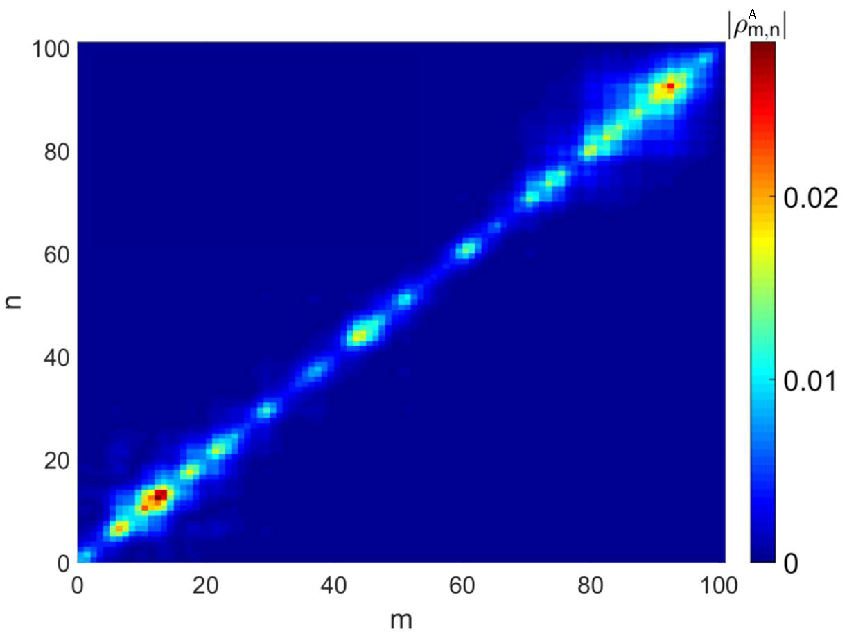
\includegraphics[width=0.5\linewidth]{anderson_rho_loc_1}}
		\hfill
		\subcaptionbox{\label{fig:anderson_rho_loc-2}}{%
			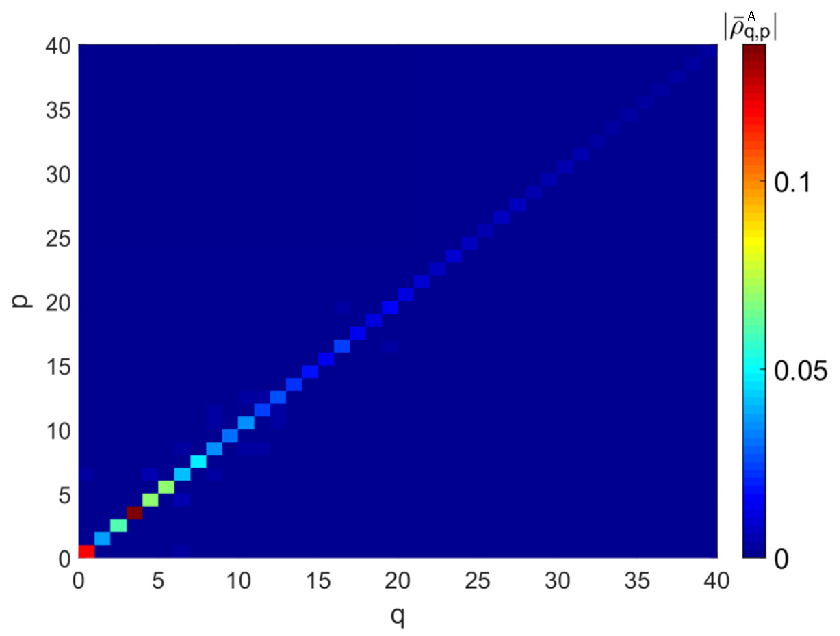
\includegraphics[width=0.5\linewidth]{anderson_rho_loc_2}}
		\hfill
	}
	\legend{}
	\caption[Асимптотическая матрица плотности с локализацией Андерсона]
	{
		Абсолютные значения асимптотической матрицы плотности \(\rho^A\) в базисе гильбертова пространства (a) и в базисе собственных состояний модели Андерсона (б) для единичной реализации беспорядка. Параметры диссипации: \(\alpha=0\) и \(l=1\). Сила пространственного беспорядка \(W=1\).
	}
	\label{fig:anderson_rho_loc}
\end{figure}

В рассматриваемой модели впервые были обнаружены асимптотические состояния со следами локализации \cite{Yusipov2017}" --- матрица плотности имеет пятнистую структуру с несколькими яркими областями локализации (рисунок \cref{fig:anderson_rho_loc-1}). 
В ходе дальнейшего исследования выяснилось, что в решении доминируют несколько локализованных мод пространственно неоднородного гамильтониана из классической модели Андерсона "--- в базисе собственных состояний гамильтониана \cref{eq:anderson_H} матрица плотности является диагональной с преобладанием собственных значений из нижней границы спектра(рисунок \cref{fig:anderson_rho_loc-2}). 
В работе было проведено дополнительное аналитическое исследование диагональных элементов матрицы плотности и установлено, что формирующие решение андерсоновские моды выбираются в соответствии с их пространственно-фазовыми свойствами, унаследованными от собственных состояний гамильтониана в пределе нулевого беспорядка, в зависимости от фазы диссипативных операторов.

Также в работе было изучено влияние фазы диссипативных операторов на локализационные свойства системы и предложен механизм управления последними \cite{Vershinina2017}. 
Метод основан на фазовых свойствах локализованных мод гамильтониана системы
Андерсона, которые являются «тёмными» состояниями синтетических диссипаторов.

Кроме этого было обнаружено, что одночастичная локализация является устойчивой к дефазирующей диссипации, которая обычно приводит системы в термализованные состояния с максимальной энтропией.

\begin{figure}[h!]
	\centerfloat{
		\hfill
		\subcaptionbox[List-of-Figures entry]{\label{fig:anderson_prb_2_1}}{%
			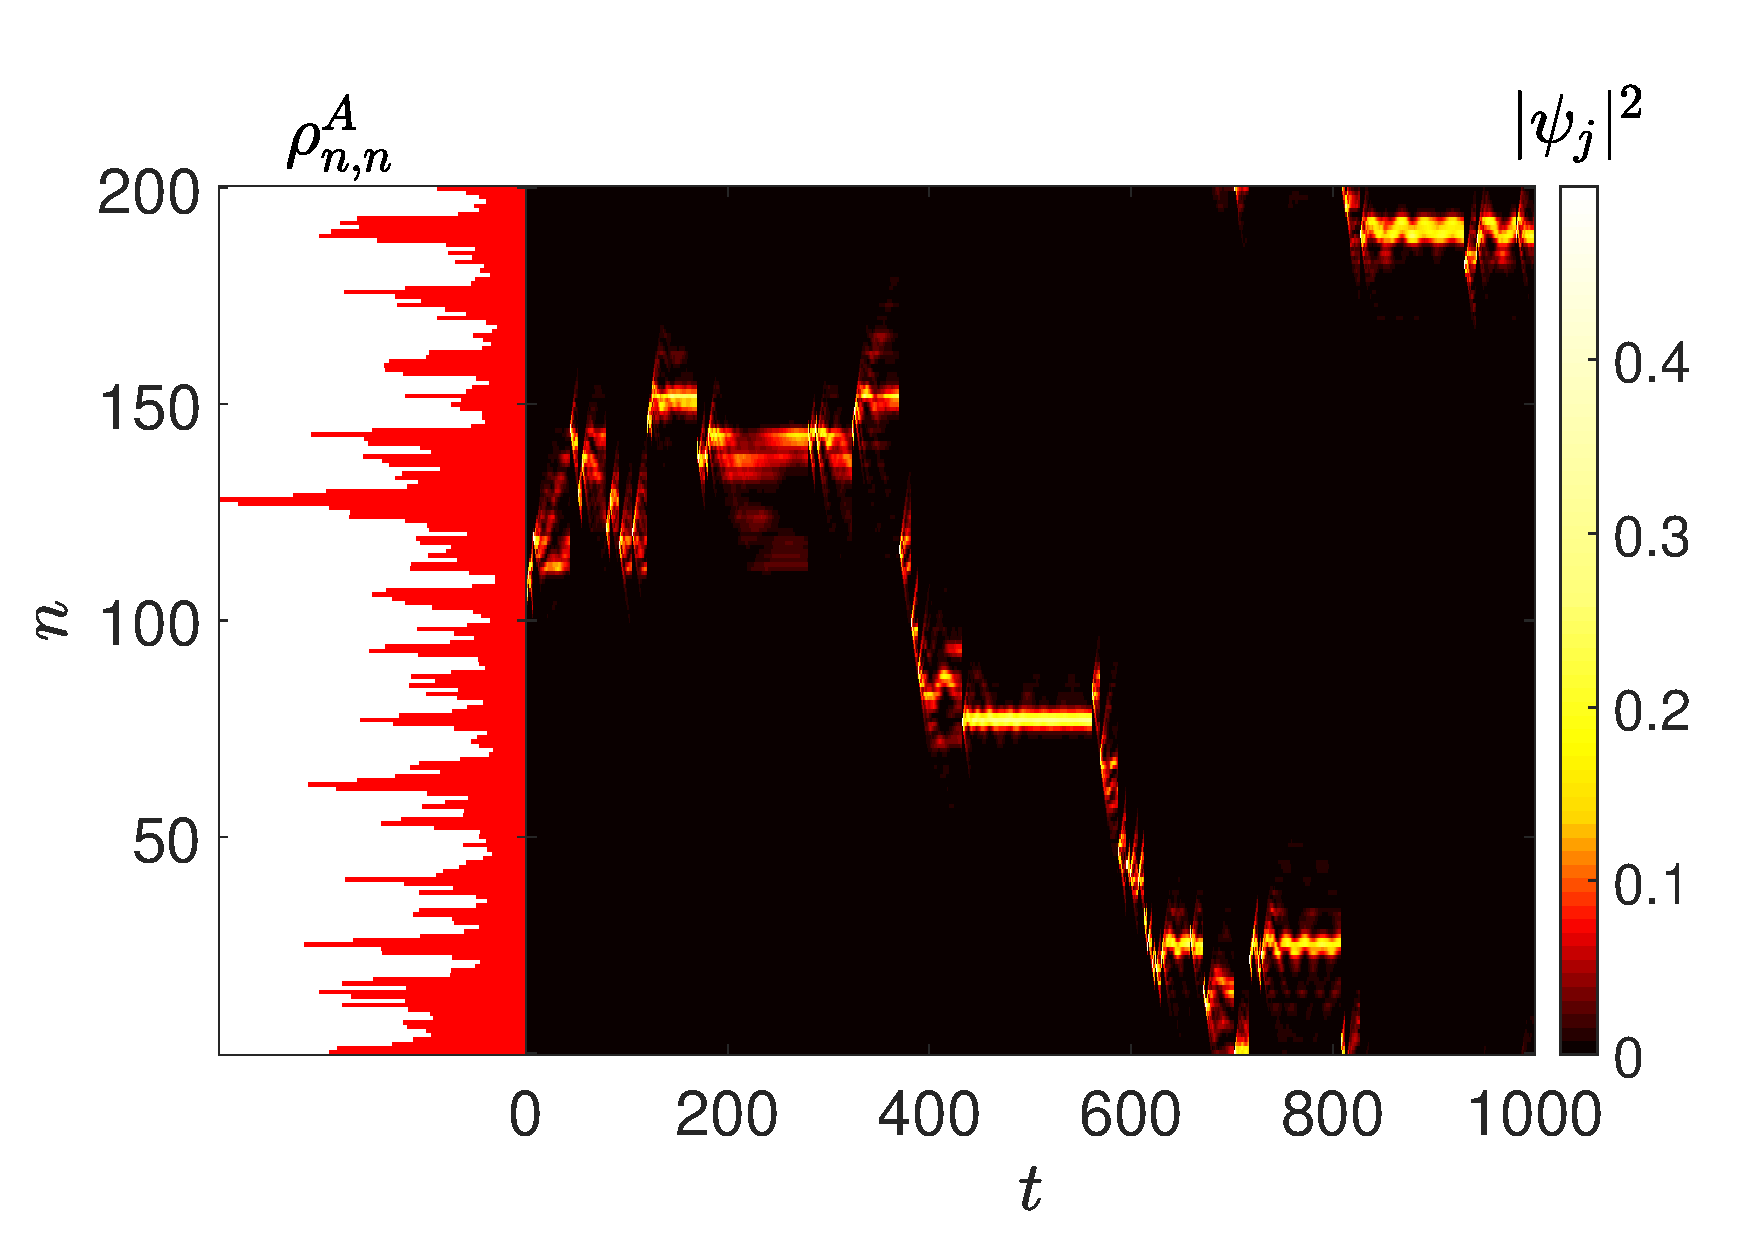
\includegraphics[width=0.5\linewidth]{anderson_prb_2_1}}
		\hfill
		\subcaptionbox{\label{fig:anderson_prb_2_2}}{%
			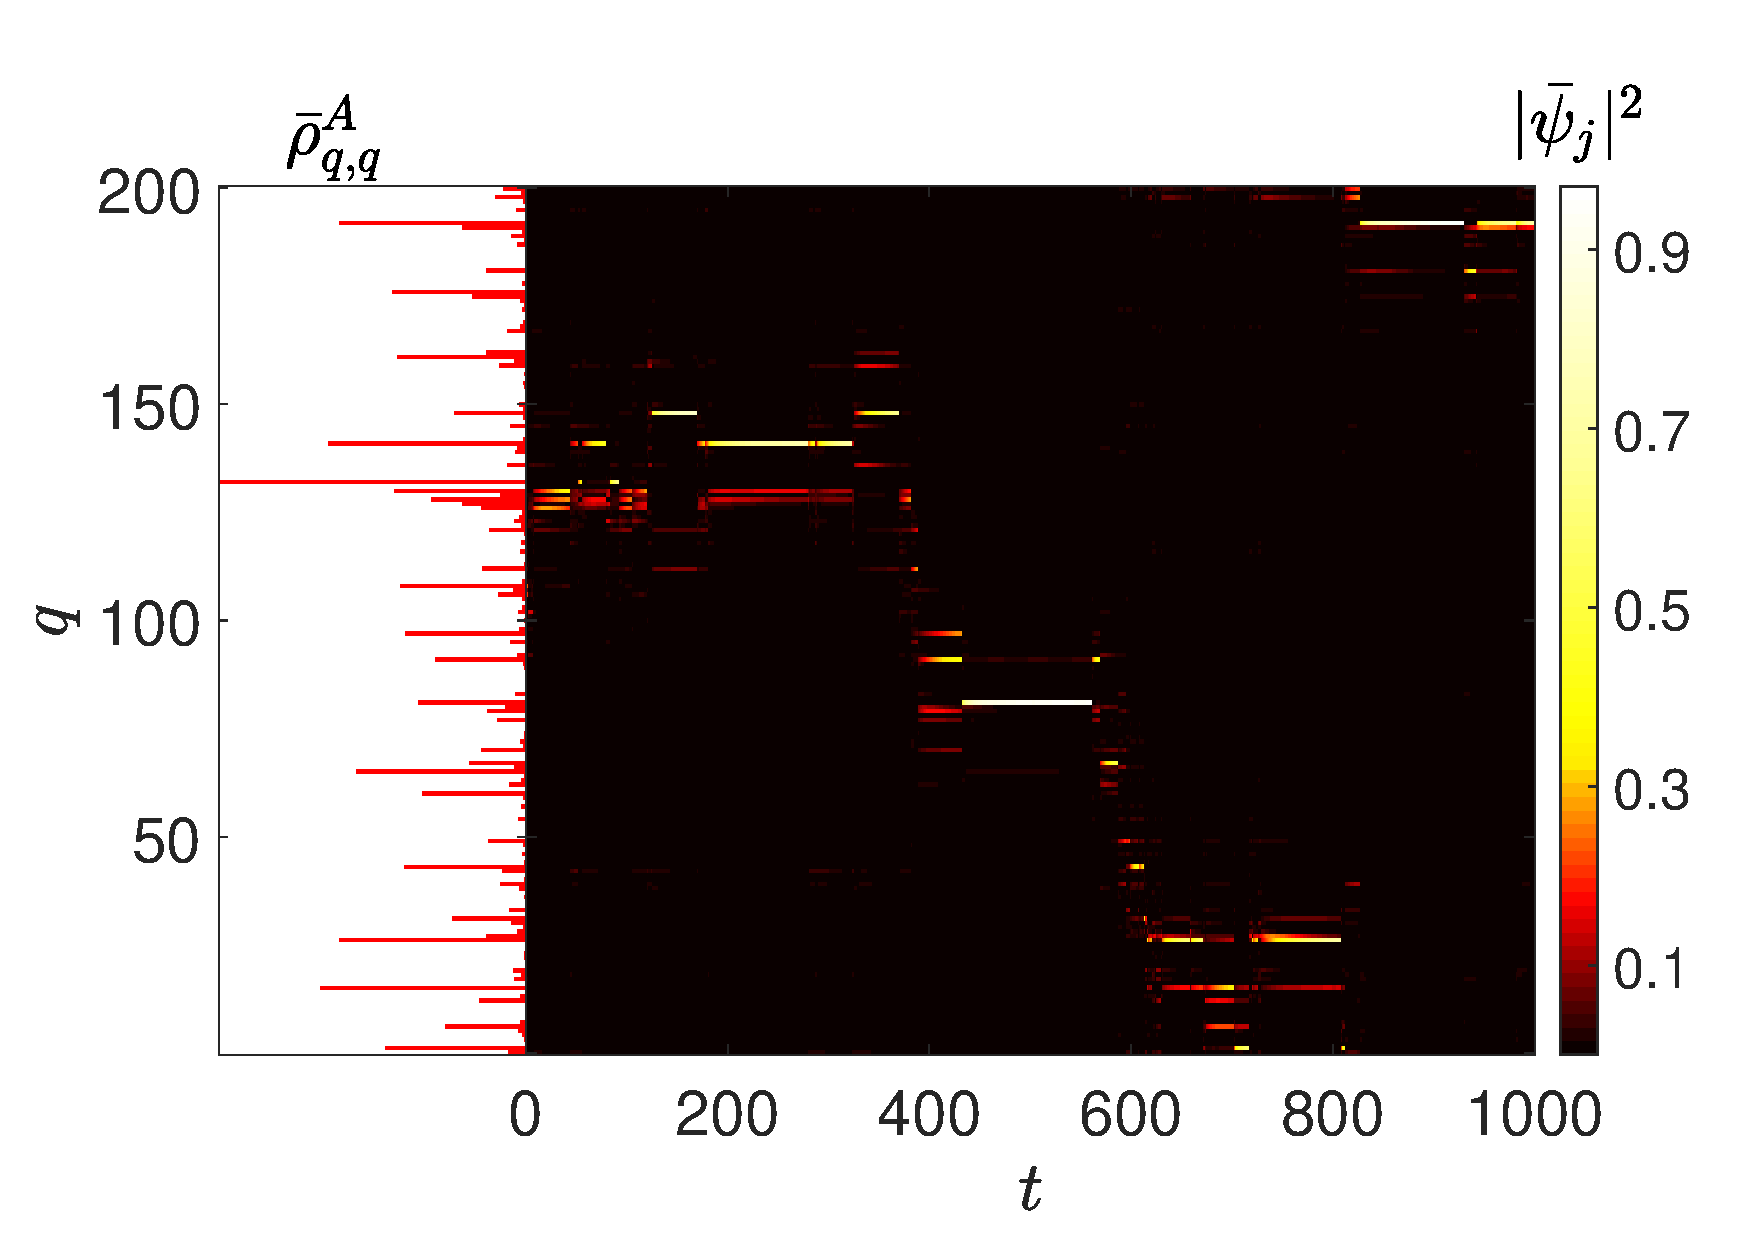
\includegraphics[width=0.5\linewidth]{anderson_prb_2_2}}
		\vfill
		\subcaptionbox[List-of-Figures entry]{\label{fig:anderson_prb_2_3}}{%
			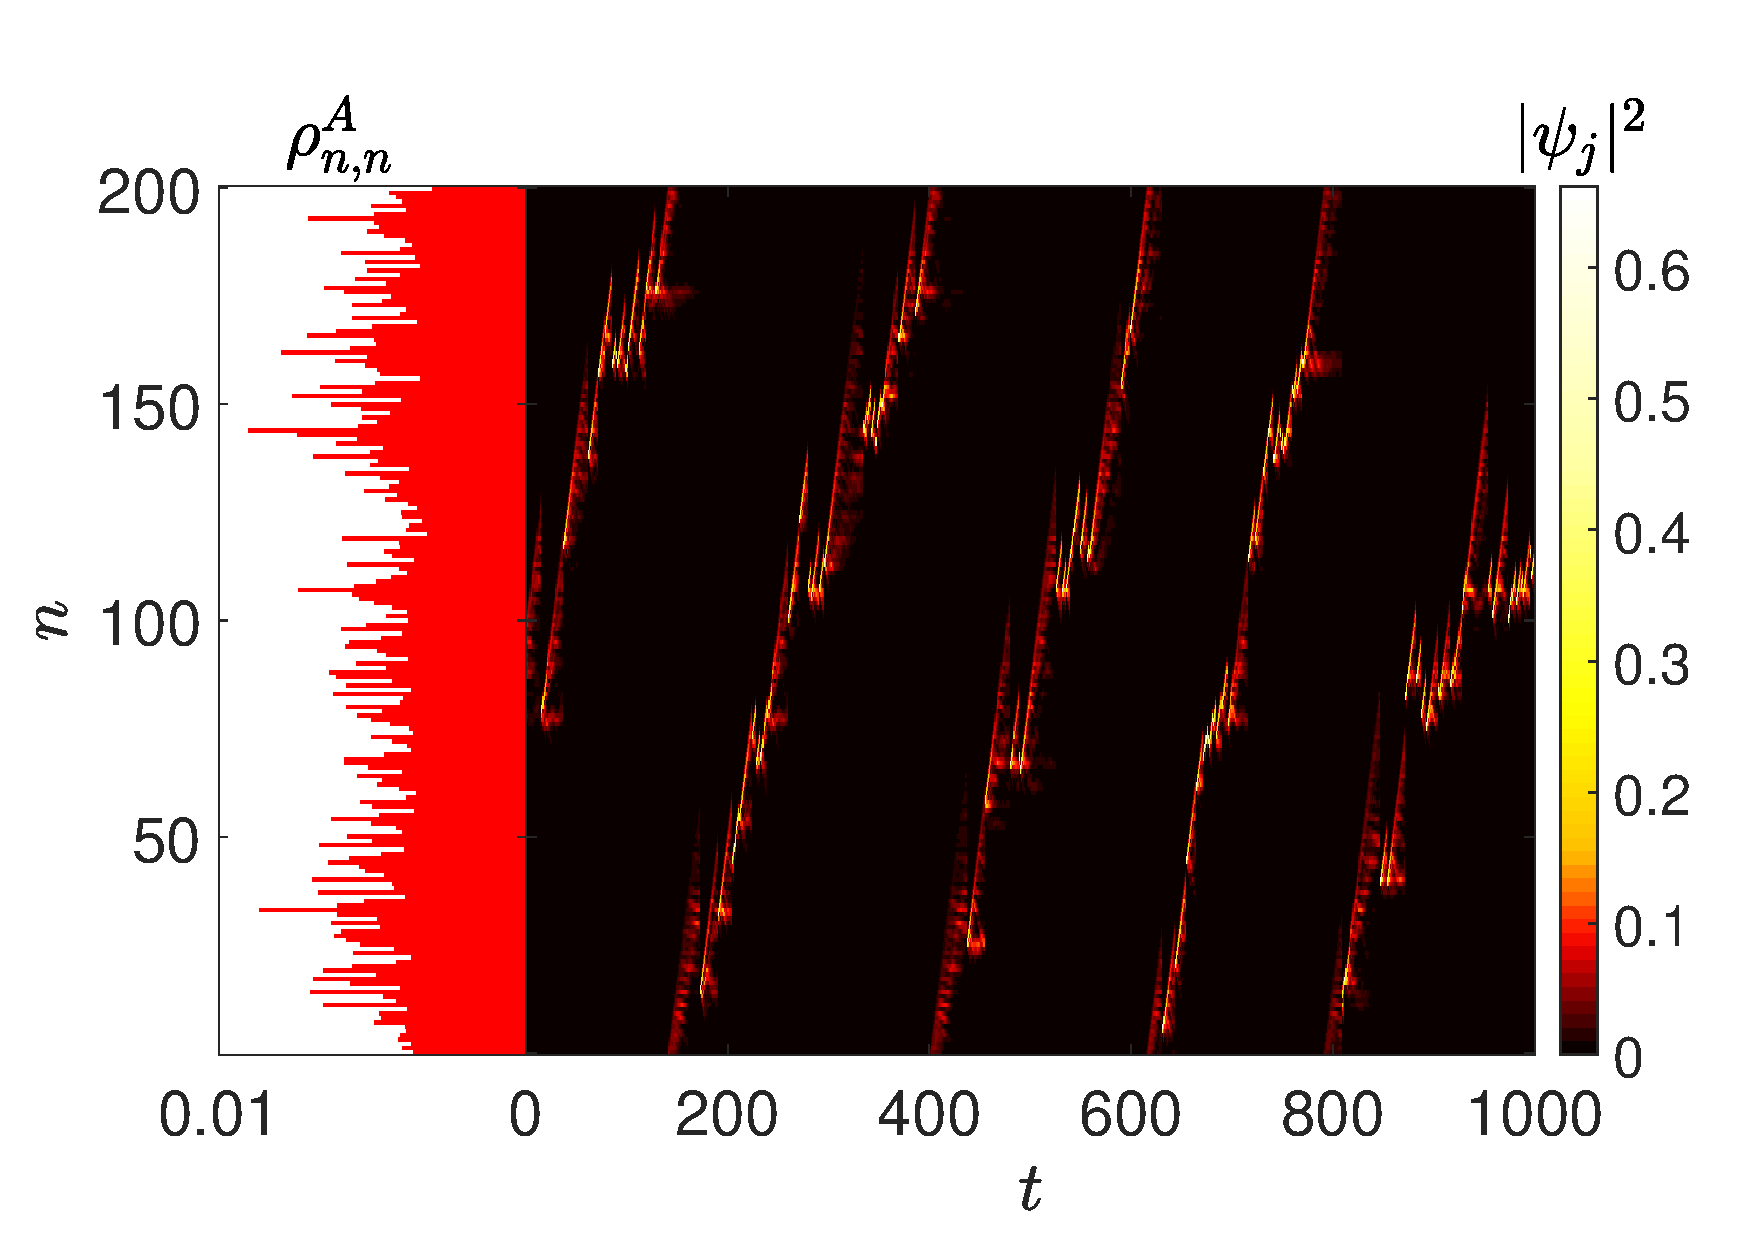
\includegraphics[width=0.5\linewidth]{anderson_prb_2_3}}
		\hfill
		\subcaptionbox{\label{fig:anderson_prb_2_4}}{%
			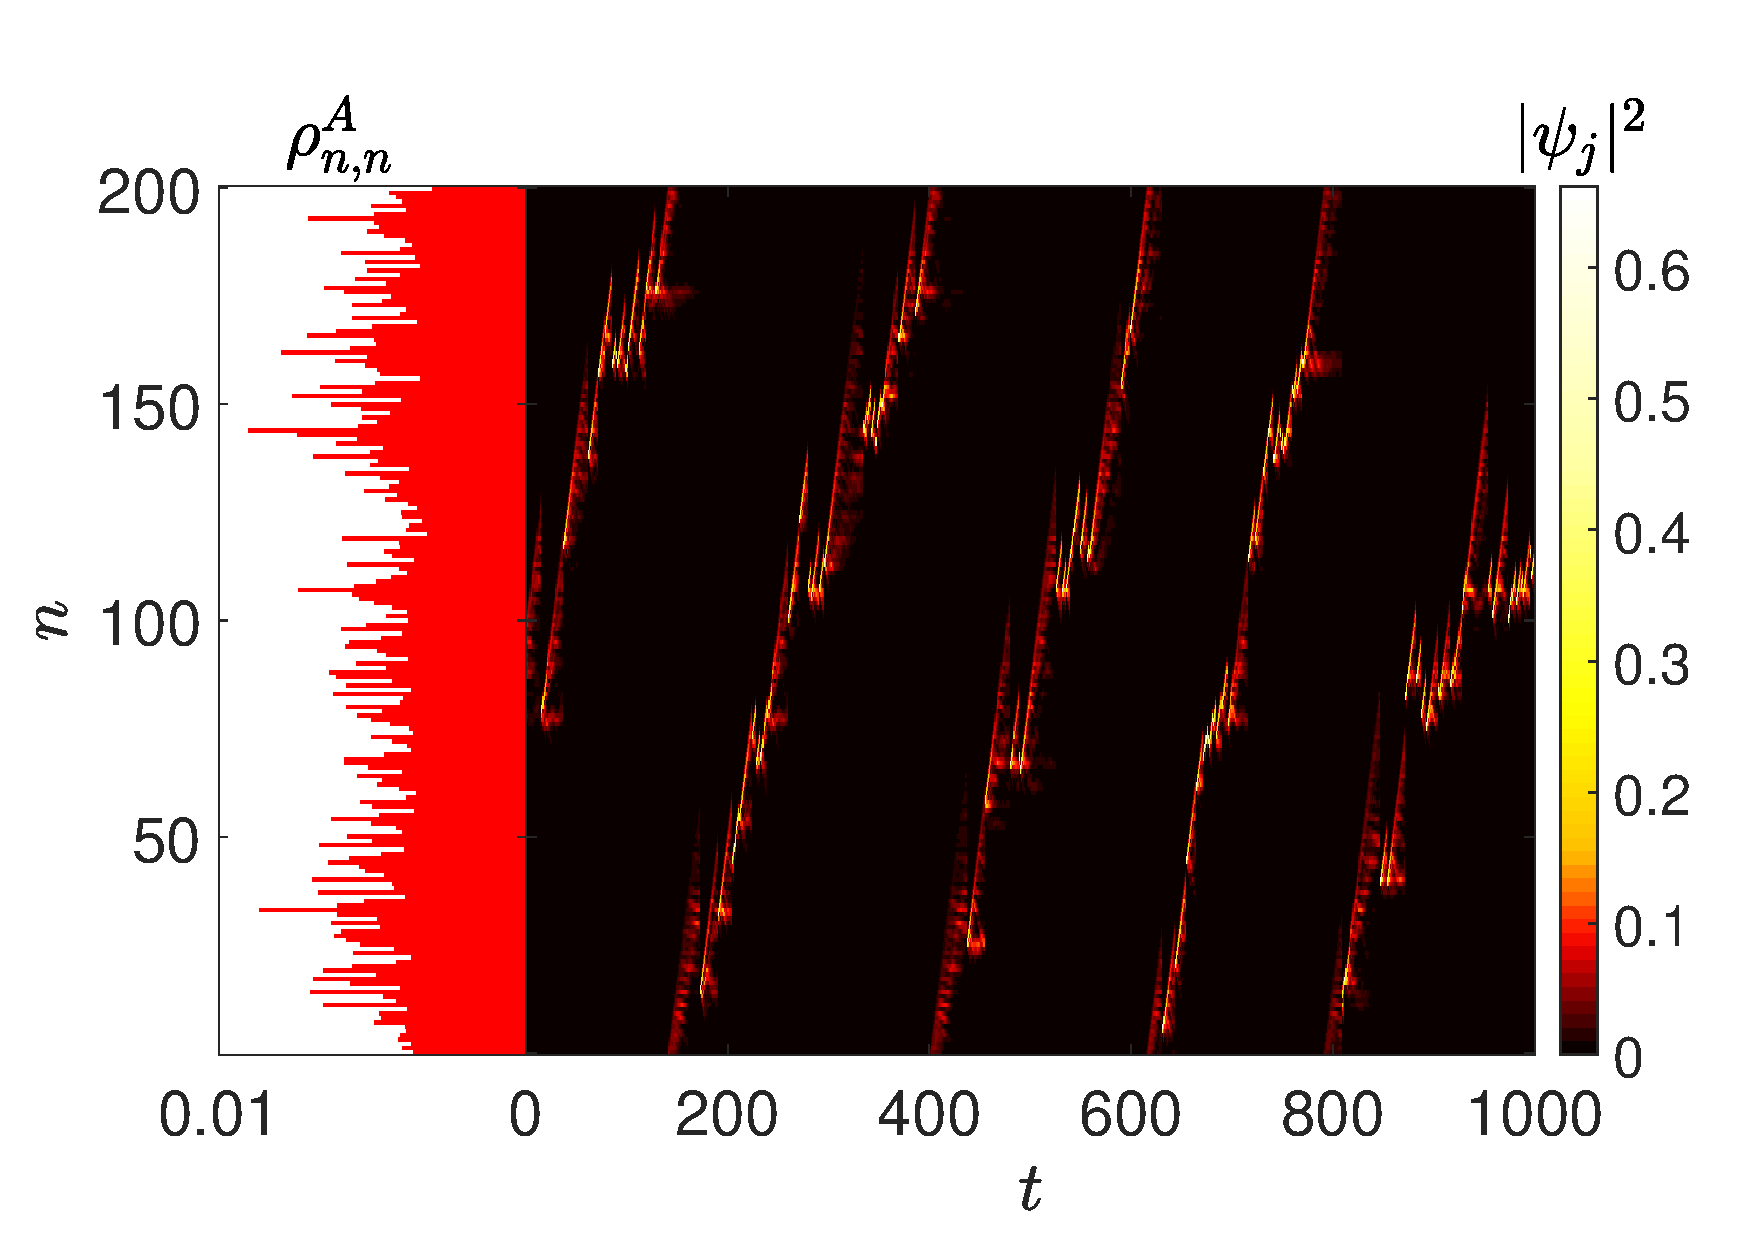
\includegraphics[width=0.5\linewidth]{anderson_prb_2_4}}
	}
	\legend{}
	\caption[Динамика квантовых траекторий на квантовых аттракторах в зависимости от параметров неэрмитовой диссипации]
	{
		Диагональные элементы асимптотической матрицы плотности (на левых вставках) и эволюция на аттракторе квадрата волновой функции отдельно взятой квантовой траектории (основные части на рисунках). (a): \(\alpha = 0\), в исходном базисе; (б): \(\alpha = 0\), в базисе Андерсоновских мод, отсортированных по центру масс; (в): \(\alpha=\frac{\pi}{4}\), в исходном базисе; (г): дефазирующая диссипация. 
	}
	\label{fig:anderson_prb_2}
\end{figure}
В данной главе при помощи метода квантовых траекторий была численно промоделирована и изучена микроскопическая динамика на аттракторах с различной степенью локализации (рисунок \cref{fig:anderson_prb_2}).
В случае нулевой фазы диссипации \cref{eq:anderson_diss_local} наблюдается прерывистая динамика состоящая из длительных циркуляций возле центров локализации и быстрых переходов между ними (рисунок \cref{fig:anderson_prb_2_1}). 
Если данную волновую функцию перевести в базис собственных состояний модели Андерсона, то можно заметить, что циркуляции происходят на модах Андерсона, которые формируют асимптотическое состояние равновесия (рисунок \cref{fig:anderson_prb_2_2}). 
Если рассмотреть ненулевую фазу неэрмитовых диссипаторов, то динамика резко изменится: для \(\alpha=\frac{\pi}{4}\) незначительные циркуляции возле центов локализации сохраняются, но самый существенный вклад в динамику вносит баллистическое распространение волновых пакетов (рисунок \cref{fig:anderson_prb_2_3}). 
При этом Дефазирующая диссипация не несёт какой-либо пространственно-временной структуры (рисунок \cref{fig:anderson_prb_2_4}).
В итоге было обнаружено, что в открытой квантовой системе с одночастичной локализацией существуют нетривиальные режимы распространения волновых пакетов за счёт взаимодействия беспорядка и диссипации. 
Квантовые траектории демонстрируют диффузионные (при которых циркуляция в Андерсоновских модах прерывается квантовыми скачками) и баллистические режимы. Управляя фазой неэрмитовых диссипаторов, можно переключать данные режимы. 
Также была изучена статистика времён между квантовыми скачками, которая сильно отличается в зависимости от типа распространения волновых пакетов в системе \cite{Yusipov2018}.






\begin{figure}[h]
	\centerfloat{
		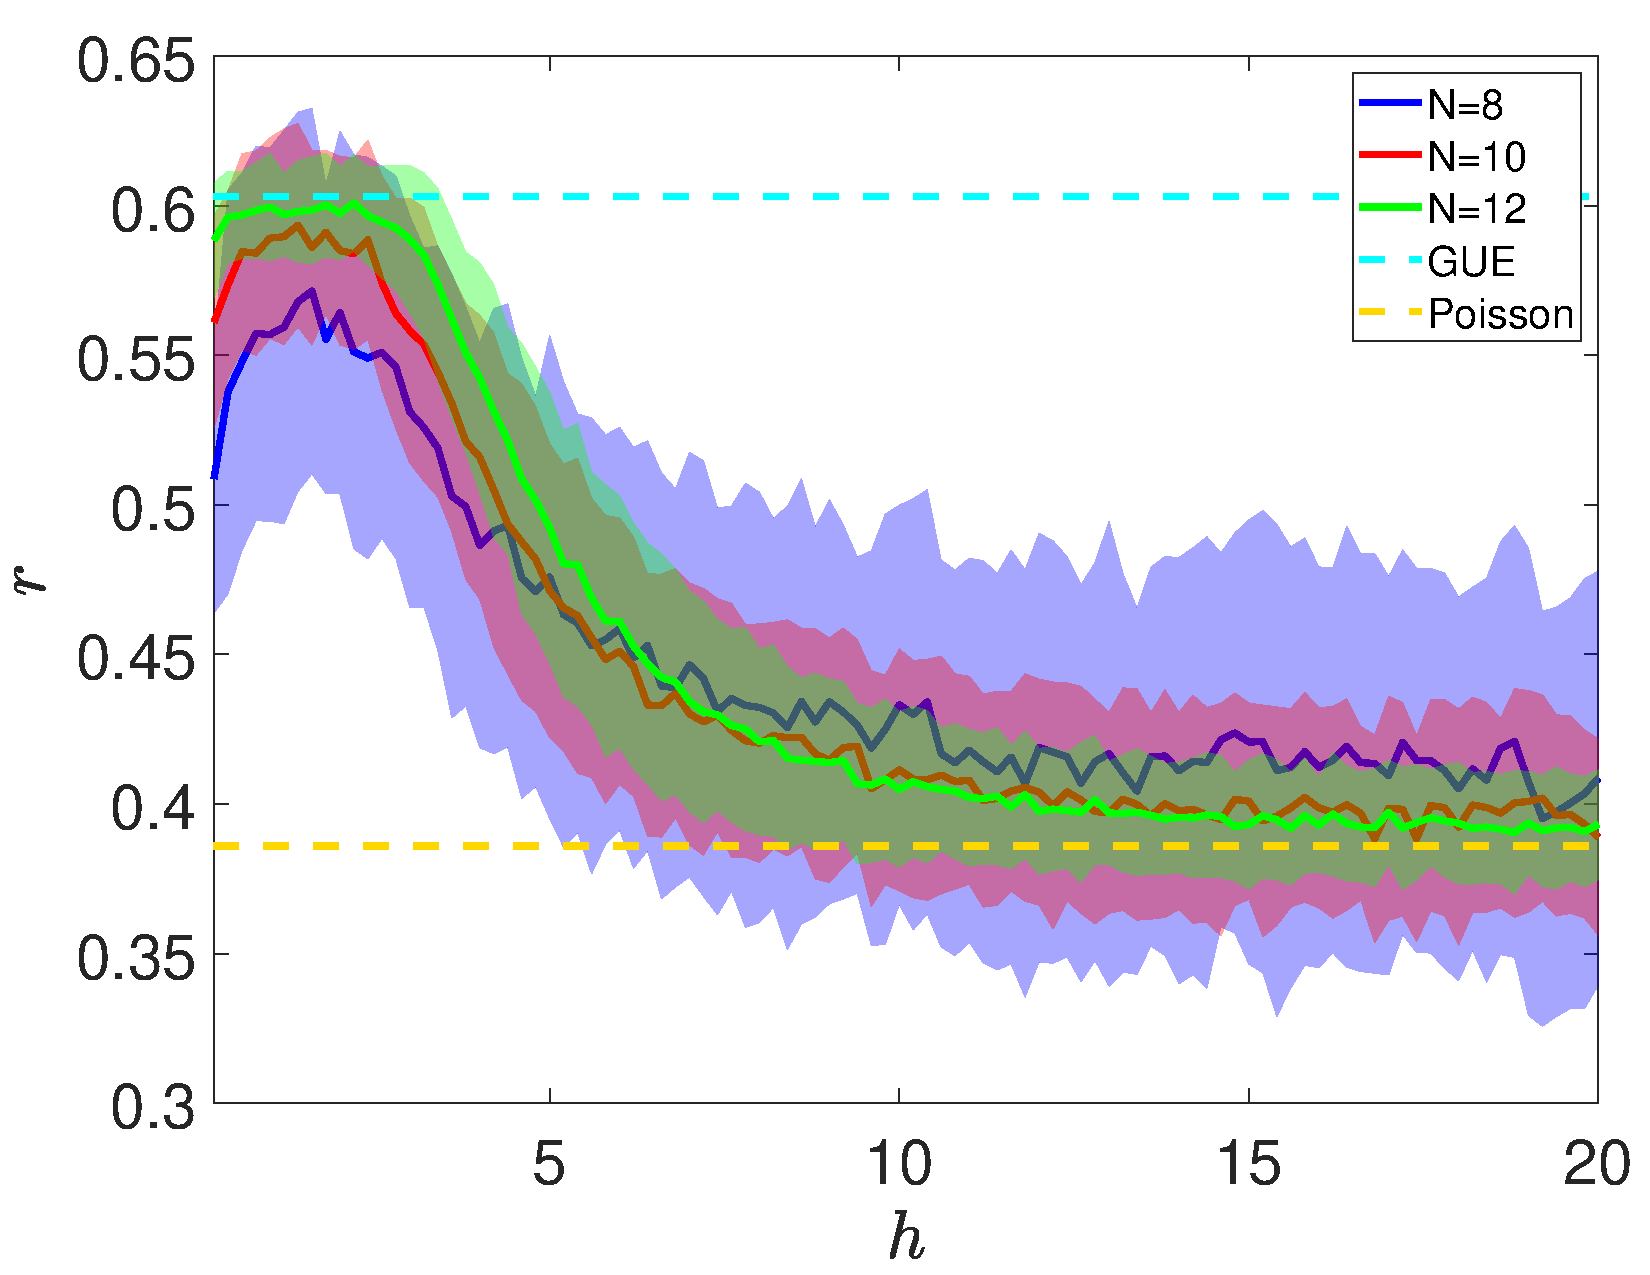
\includegraphics[scale=0.3]{mbl_ratio}
	}
	\caption[Соотношение последовательных уровней для асимптотической матрицы плотности в зависимости от силы беспорядка в системе]{
		Соотношение последовательных уровней собственных значений асимптотической матрицы плотности \(\rho^A\) в зависимости от силы беспорядка \(h\). Сплошными линиями обозначено усреднённое значение \(r\) по \(N_r=100\) реализациям беспорядка для каждого значения \(h\). Области соответствующего цвета обозначают стандартное отклонение распределения \(r\). Пунктирные линии соответствуют значениям \(r\), характерным для случайных величин с распределением Пуассона (регулярная динамика, локализация) и случайных матриц из гауссова унитарного ансамбля GUE (хаос, отсутствие локализации).
	}
	\label{fig:mbl_ratio}
\end{figure}

Помимо одночастичной локализации в данной главе было численно промоделировано и изучено явление многочастичной локализации (MBL) в открытых квантовых системах. Соответствующая математическая модель задаётся уравнением Линдблада \cref{eq:GKSL_base} с многочастичным гамильтонианом для \(\frac{N}{2}\) бесспиновых фермионов на решётке размером \(N\): 
\begin{equation}
\label{eq:mbl_H}
\begin{gathered}
H = \sum_{n=1}^{N} h_n b^{\dagger}_n b_n + \sum_{n=1}^{N-1} b^{\dagger}_n b_n b^{\dagger}_{n+1} b_{n+1} - \sum_{n=1}^{N-1} \left( b^{\dagger}_n b_{n+1} + b^{\dagger}_{n+1} b_n \right) ,
\end{gathered}
\end{equation}
где \(b_n\) и \(b^{\dagger}_n\) "--- операторы уничтожения и создания фермиона на \(n\)-ом сайте решётки соответственно, \(b^{\dagger}_n b_n\) "--- оператор числа частиц на сайте \(n\).
В каждом узле решётки на фермионы действуют случайные потенциалы \(h_n\) (первое слагаемое в правой части). Фермионы, которые находятся в соседних сайтах решётки, взаимодействуют между собой (второе слагаемое в правой части). Третье слагаемое в правой части отвечает за перемещение фермионов между сайтами решётки. Значения случайных потенциалов \(h_n\) равномерно распределены в интервале \(\left[-h, h \right]\).
Как и в одночастичной модели, рассматривается специальный тип диссипации:
\begin{equation}
\label{eq:mbl_diss_diehl}
\begin{gathered}
V^l_k = ( b^\dagger_k + b^\dagger_{k+1}) \left( b_k - b_{k+1} \right),
\end{gathered}
\end{equation}
который приводит систему в состояние со следами многочастичной локализации. 
Для численной оценки многочастичной локализации в открытых квантовых системах были предложены три численных характеристики:
\begin{enumerate}[beginpenalty=10000] % https://tex.stackexchange.com/a/476052/104425
	\item статистика дисбаланса (величина, которая может быть измерена в реальном физическом эксперименте);
	\item энтропия запутанности операторного пространства (указывает на различия между эргодической фазой и многочастичной локализацией как в асимптотическом пределе, так и во время релаксации к нему);
	\item соотношение последовательных уровней \(r\) собственных значений асимптотической матрицы плотности (рисунок \ref{fig:mbl_ratio}), которое связывает явление многочастичной локализации с теорией случайных матриц и квантового хаоса.
\end{enumerate} 

В итоге было обнаружено, что физически реализуемая неэрмитовая диссипация \cref{eq:mbl_diss_diehl}, нетривиально действующая на соседних сайтах многочастичной системы пытается построить классические и квантовые корреляции между далеко расположенными сайтами, и даже дефазирующая диссипация не может их разрушить \cite{Vakulchyk2018}. 
В то же время механизмы MBL, индуцированные гамильтонианом, пытаются ограничить корреляции длиной локализации. 
В результате баланса между этими факторами возникает асимптотическое состояние со следами локализации, которые можно численно детектировать предложенными в работе характеристиками. 

Результаты данной главы опубликованы в работах \cite{Yusipov2017, Vershinina2017, Yusipov2018, Vakulchyk2018, sessiann_2017, rf_2017, shilnikov_2017}.

\FloatBarrier
\pdfbookmark{Заключение}{conclusion}                                  % Закладка pdf
В \underline{\textbf{заключении}} приведены основные результаты работы, которые заключаются в следующем:
%% Согласно ГОСТ Р 7.0.11-2011:
%% 5.3.3 В заключении диссертации излагают итоги выполненного исследования, рекомендации, перспективы дальнейшей разработки темы.
%% 9.2.3 В заключении автореферата диссертации излагают итоги данного исследования, рекомендации и перспективы дальнейшей разработки темы.
\begin{enumerate}[beginpenalty=10000] % https://tex.stackexchange.com/a/476052/104425
	\item Разработан программный комплекс \cite{prog1}, осуществляющий численное моделирование открытых квантовых систем с большим числом состояний, включающий в себя возможность анализа отдельных квантовых траекторий, поиск асимптотических состояний системы путём численного интегрирования (при наличии модуляции в системе) или поиска собственного состояния системы.
	\item Обнаружена и численно исследована математическая модель открытой квантовой системы с признаками одночастичной локализации в асимптотических состояниях \cite{Yusipov2017}. 
	Разработан метод управления локализационными свойствами получаемого квантового аттрактора \cite{Vershinina2017} "--- асимптотическое состояние может быть локализовано в любом месте спектра гамильтониана, за счёт управляемой синтетической диссипации.
	В рассматриваемой модели изучены характеристики волновых пакетов отдельных квантовых траекторий в асимптотическом режиме \cite{Yusipov2018}.
	\item Численно исследована математическая модель открытой квантовой системы с признаками многочастичной локализации в асимптотических состояниях. Предложены количественные критерии данного явления \cite{Vakulchyk2018}.
	\item В ходе численного анализа модели открытого периодически модулируемого квантового димера обнаружен квантовый аналог бифуркации Неймарка"--~Сакера (рождение тора из-за неустойчивости предельного цикла) \cite{Yusipov2019_1}.
	\item Разработан и программно реализован \cite{prog1} алгоритм нахождения старшего квантового показателя Ляпунова, основанный на методе квантовых траекторий. Данная разработка позволяет выявить сложную структуру регулярных и хаотических областей, дать количественную оценку диссипативному квантовому хаосу. Как и классический старший показатель Ляпунова, его квантовый аналог становится положительным в случае хаотической динамики системы \cite{Yusipov2019_2}.
	\item Предложен экспериментально осуществимый подход к обнаружению регулярных и хаотических режимов в определённом классе математических моделей открытых квантовых систем на основе анализа статистики распределения времени ожидания фотона. При переходе в режим квантового хаоса режиме появляется степенная асимптотика в распределении времени ожидания фотона \cite{Yusipov2020}. Также численно исследованы математические модели со спин-фотонным взаимодействием, позволяющим регулировать динамику в системе \cite{Yusipov2021}.
\end{enumerate}


\pdfbookmark{Литература}{bibliography}                                % Закладка pdf

\ifdefmacro{\microtypesetup}{\microtypesetup{protrusion=false}}{} % не рекомендуется применять пакет микротипографики к автоматически генерируемому списку литературы
\urlstyle{rm}                               % ссылки URL обычным шрифтом
\ifnumequal{\value{bibliosel}}{0}{% Встроенная реализация с загрузкой файла через движок bibtex8
  \renewcommand{\bibname}{\large \bibtitleauthor}
  \nocite{*}
  \insertbiblioauthor           % Подключаем Bib-базы
  %\insertbiblioexternal   % !!! bibtex не умеет работать с несколькими библиографиями !!!
}{% Реализация пакетом biblatex через движок biber
  % Цитирования.
  %  * Порядок перечисления определяет порядок в библиографии (только внутри подраздела, если `\insertbiblioauthorgrouped`).
  %  * Если не соблюдать порядок "как для \printbibliography", нумерация в `\insertbiblioauthor` будет кривой.
  %  * Если цитировать каждый источник отдельной командой --- найти некоторые ошибки будет проще.
  %
  %% authorvak
  %\nocite{vakbib1}%
  %\nocite{vakbib2}%
  %
  %% authorwos
  \nocite{Yusipov2017}%
  \nocite{Vershinina2017}%
  \nocite{Yusipov2018}%
  \nocite{Vakulchyk2018}%
  \nocite{Yusipov2019_2}%
  \nocite{Yusipov2019_1}%
  \nocite{Yusipov2020}%
  \nocite{Liniov2019}%
  %
  %% authorscopus
  %\nocite{scbib1}%
  %
  %% authorpathent
  %\nocite{patbib1}%
  %
  %% authorprogram
  \nocite{prog1}%
  %
  %% authorconf
  \nocite{sessiann_2017}%
  \nocite{rf_2017}%
  \nocite{sfy_2017}%
  \nocite{shilnikov_2017}%
  \nocite{sessiann_2018}%
  \nocite{rf_2018}%
  \nocite{nnnph_2018}%
  \nocite{physcon_2019}%
  \nocite{rf_2020}%
  %\nocite{confbib1}%
  %\nocite{confbib2}%
  %
  %% authorother
  %\nocite{bib1}%
  %\nocite{bib2}%

  \ifnumgreater{\value{usefootcite}}{0}{
    \begin{refcontext}[labelprefix={}]
      \ifnum \value{bibgrouped}>0
        \insertbiblioauthorgrouped    % Вывод всех работ автора, сгруппированных по источникам
      \else
        \insertbiblioauthor      % Вывод всех работ автора
      \fi
    \end{refcontext}
  }{
  \ifnum \totvalue{citeexternal}>0
    \begin{refcontext}[labelprefix=A]
      \ifnum \value{bibgrouped}>0
        \insertbiblioauthorgrouped    % Вывод всех работ автора, сгруппированных по источникам
      \else
        \insertbiblioauthor      % Вывод всех работ автора
      \fi
    \end{refcontext}
  \else
    \ifnum \value{bibgrouped}>0
      \insertbiblioauthorgrouped    % Вывод всех работ автора, сгруппированных по источникам
    \else
      \insertbiblioauthor      % Вывод всех работ автора
    \fi
  \fi
  %  \insertbiblioauthorimportant  % Вывод наиболее значимых работ автора (определяется в файле characteristic во второй section)
  \begin{refcontext}[labelprefix={}]
      \insertbiblioexternal            % Вывод списка литературы, на которую ссылались в тексте автореферата
  \end{refcontext}
  % Невидимый библиографический список для подсчёта количества внешних публикаций
  % Используется, чтобы убрать приставку "А" у работ автора, если в автореферате нет
  % цитирований внешних источников.
  \printbibliography[heading=nobibheading, section=0, env=countexternal, keyword=biblioexternal, resetnumbers=true]%
  }
}
\ifdefmacro{\microtypesetup}{\microtypesetup{protrusion=true}}{}
\urlstyle{tt}                               % возвращаем установки шрифта ссылок URL
